\documentclass[a4paper,12pt]{article} 
\usepackage[T2A]{fontenc}			
\usepackage[utf8]{inputenc}			
\usepackage[english,russian]{babel}	
\usepackage{amsmath,amsfonts,amssymb,amsthm,mathrsfs,mathtools} 
\usepackage{cancel}
\usepackage{multirow}
\usepackage[colorlinks, linkcolor = blue]{hyperref}
\usepackage{upgreek}\usepackage[left=2cm,right=2cm,top=2cm,bottom=3cm,bindingoffset=0cm]{geometry}
\usepackage{graphicx,wrapfig,subfig}
\usepackage{tikz}
\usepackage{pgfplots}
\usepackage{xcolor}
\author{Дорогинин Д.В.\\
Группа Б02-825}
\title{3.5.1. Изучение плазмы газового разряда в неоне.}
\date{}


\graphicspath{ {images/} }
\usepackage{multicol}
\setlength{\columnsep}{2cm}


\begin{document}

\begin{titlepage}
	\centering
	\vspace{5cm}
	{\scshape\LARGE Московский физико-технический институт \par}
	\vspace{4cm}
	{\scshape\Large Лабораторная работа 4.2.1 \par}
	\vspace{1cm}
	{\huge\bfseries Кольца Ньютона. \par}
	\vspace{1cm}
	\vfill
\begin{flushright}
	{\large выполнил студент 924 группы ФОПФ}\par
	\vspace{0.3cm}
	{\LARGE Панферов Андрей}
\end{flushright}
	

	\vfill

% Bottom of the page
	Долгопрудный, 2021 г.
\end{titlepage}

\textbf{Цель работы}: Познакомиться с явлением интерференции в тонких плёнках (полосы равной толщины) на примере колец Ньютона и с методикой интерференционных измерений кривизны стеклянной поверхности.

\textbf{В работе используются}: Измерительный микроскоп с опак-иллюминатором, плоско-выпуклая линза; пластинка из чёрного стекла, ртутная лампа типа ДРШ, щель, линзы, призма прямого зрения, объектная шкала.

\section*{Теоретическое введение}
	
	\begin{wrapfigure}{l}{0.35\linewidth} 
		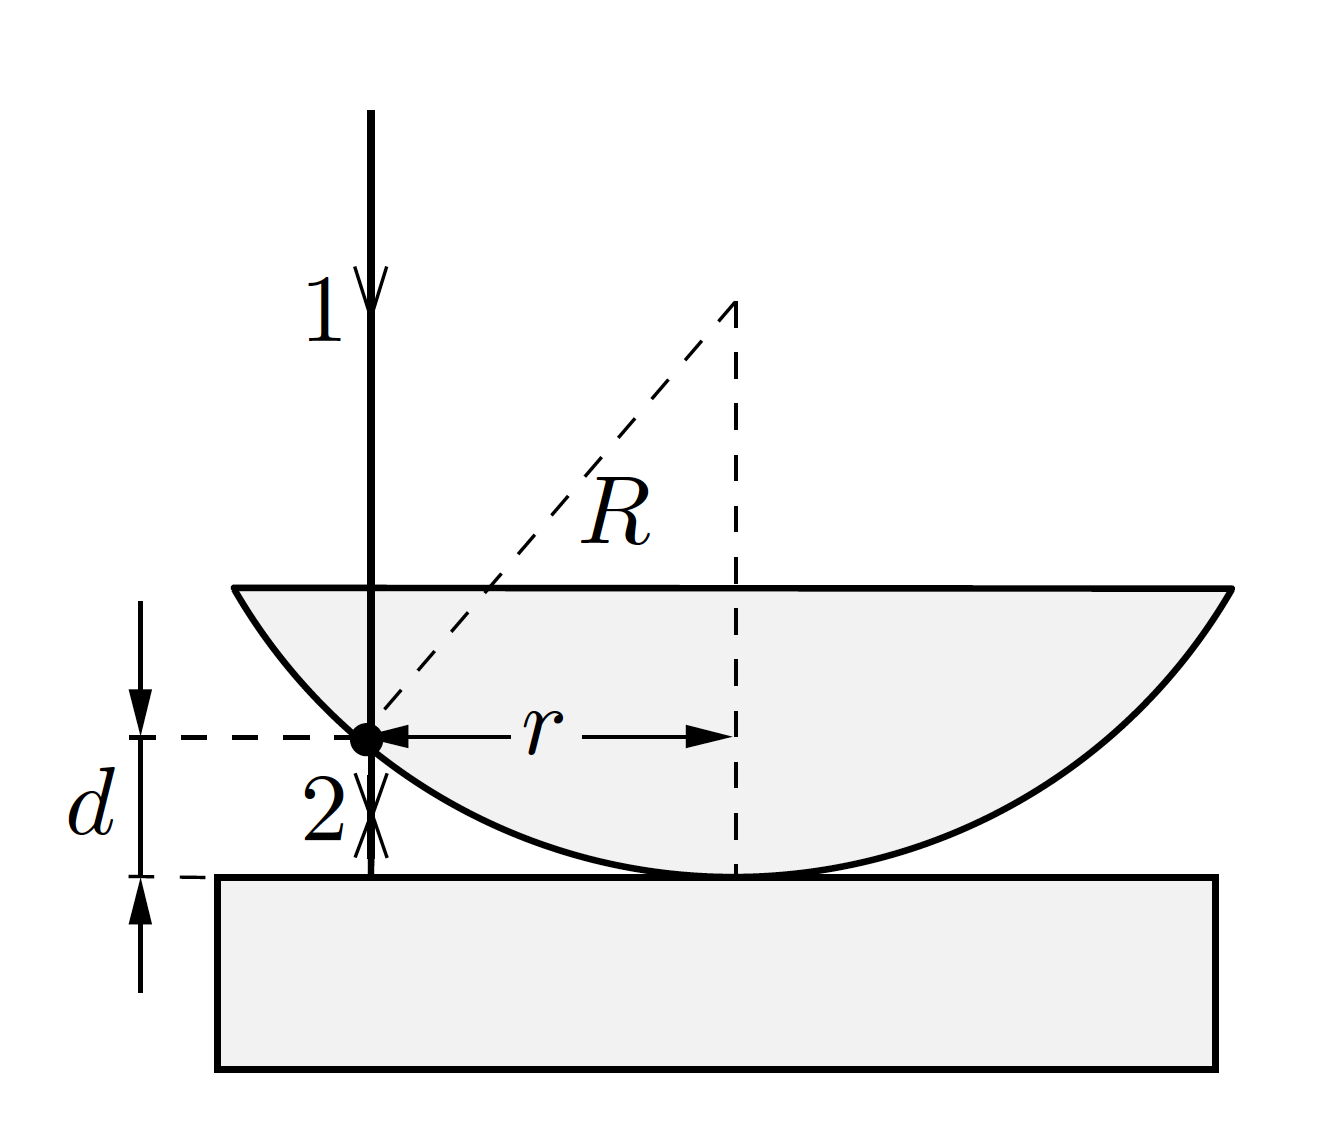
\includegraphics[width=\linewidth]{ring}
		\caption{Экспериментальная установка}
		\label{ring}
	\end{wrapfigure}

	Этот классический опыт используется для определения радиуса кривизны сферических поверхностей линз. В этом опыте наблюдается интерференция волн, отражённых от границ тонкой воздушной прослойки, образованной сферической поверхностью линзы и плоской стеклянной пластиной. При нормальном падении света (рис. \ref{ring}) интерференционные полосы локализованы на сферической поверхности и являются полосами равной толщины.
	
	Геометрическая разность хода между интерферирующими лучами равна удвоенной толщине воздушного зазора $ 2d $ в данном месте. Для точки на сферической поверхности, находящейся на расстоянии $ r $ от оси системы, имеем $ r^2 = R^2 - (R - d)^2 = 2Rd - d^2 $, где $ R $ --- радиус кривизны сферической поверхности (рис. \ref{ring}).
	
	При $ R \gg d $ получим$  d = r^2/2R $. С учётом изменения фазы на $ \pi $ при отражении волны от оптически более плотной среды (на границе воздух-стекло) получим \textbf{оптическую разность хода интерферирующих лучей}:
	
	\begin{equation}\label{r_m}
	\Delta = \dfrac{\lambda}{2} + 2d = \dfrac{r^2}{2R} + \dfrac{\lambda}{2}
	\end{equation}
	
	Из условия интерференционного минимума $ \Delta = \dfrac{(2m +1)\lambda}{2}, \; m =0, 1, 2.. $ получим радиусы темных колец $ r_m $, а из аналогичного условия максимума $ \Delta = m \lambda $ радиусы светлых $ r_m' $ :
	
	\begin{equation}\label{r_m'}
	r_m = \sqrt{m \lambda R}, \qquad 	r_m' = \sqrt{\dfrac{(2m-1) \lambda R}{2}}
	\end{equation}
	
	\section{Экспериментальная установка}

Схема экспериментальной установки приведена на рис. \ref{lab}. Опыт выполняется с помощью измерительного микроскопа.
На столик микроскопа помещается держатель с полированной пластинкой из
чёрного стекла. На пластинке лежит исследуемая линза.

\newpage

	\begin{wrapfigure}{r}{0.5\linewidth} 
	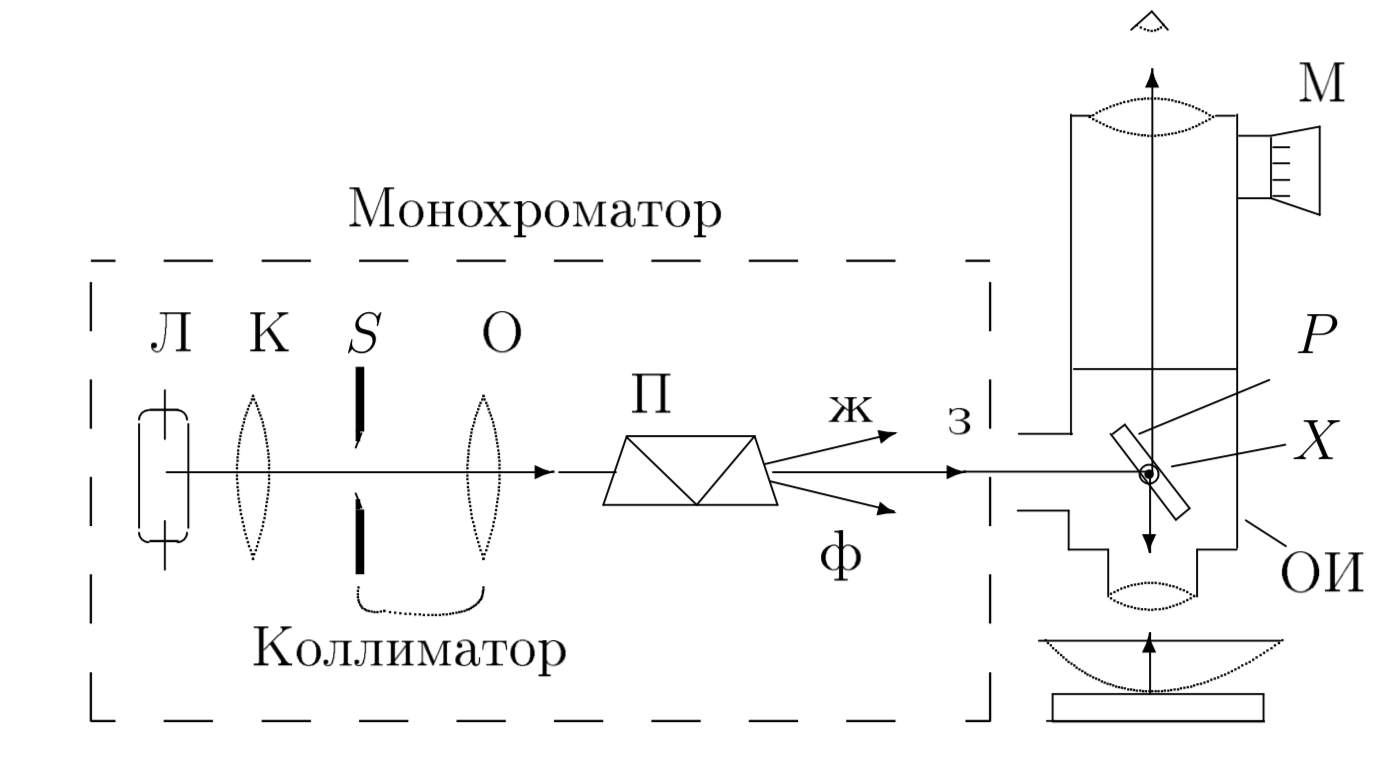
\includegraphics[width=\linewidth]{lab}
	\caption{Экспериментальная установка}
	\label{lab}
\end{wrapfigure}

	Источником света служит ртутная лампа, находящаяся в защитном кожухе. Для получения монохроматического света применяется призменный монохроматор, состоящий из конденсора $ К $, коллиматора (щель $ S $ и объектив $ О $) и призмы прямого зрения $ П $. Эти устройства с помощью рейтеров располагаются на оптической скамье. Свет от монохроматора попадает на расположенный между объективом и окуляром микроскопа опак-иллюминатор (ОИ)  специальное устройство, служащее для освещения объекта при работе в отражённом свете. Внутри опак-иллюминатора находится полупрозрачная стеклянная пластинка P, наклоненная под углом $ 45^\circ $ к оптической оси микроскопа. Свет частично отражается от этой пластинки, проходит через объектив микроскопа и попадает на исследуемый объект. Пластинка может поворачиваться вокруг горизонтальной оси $ X $, опак-иллюминатор вокруг вертикальной оси.

	Столик микроскопа может перемещаться в двух взаимно перпендикулярных направлениях помощью винтов препаратоводителя. Отсчетный крест окулярной шкалы перемещается перпендикулярно оптической оси с помощью микрометрического винта $ М $.
	
	Оптическая схема монохроматора позволяет получить в плоскости входного окна опак-иллюминатора достаточно хорошо разделённые линии спектра ртутной лампы. Изображение щели $ S $ фокусируется на поверхность линзы объективом микроскопа, т.е. точка источника и точка наблюдения спектра совпадают.Интерференционная картина не зависит от показателя преломления линзы и определяется величиной зазора между линзой и пластинкой (кольца равной толщины).

	Сначала микроскоп настраивается на кольца Ньютона в белом свете (свете ртутной лампы), затем при помощи монохроматора выделить из спектра яркую зелёную линию и провести измерения диаметров колец в монохроматическом свете. 

\section*{Ход работы}
	
	После настройки микроскопа проведем измерения диаметров колец Ньютона. Измерения будем проводить в безразмерных единицах окулярной шкалы, переведённых затем в реальную величину с помощью калиброванной объектной шкалы. 
	
	
	Оценим систематическую погрешность измерения величин на окуляре как $ \sigma_l = 0,02 $ (из-за цены деления).
	
	C помощью призмы выделим зеленый свет из спектра лампы ($ \lambda_{green} = 546 $ нм).
	
	Будем последовательно измерять координаты экстремумов $ l $. Результаты занесем в Tаблицу \ref{table::rings}.
	
\newpage
\begin{table}
\begin{minipage}{0.5\textwidth}
\begin{tabular}{|l|l|l|l|l|}
\hline
m      & $l_{dark}$ & $l_{light}$ & $r_{dark}^2$ & $r_{light}^2$ \\ \hline
center & 0.85           & 0.85            & 0                         & 0                          \\ \hline
1      & 1.34           & 1.07            & 0.2401                    & 0.0484                     \\ \hline
2      & 1.81           & 1.62            & 0.9216                    & 0.5929                     \\ \hline
3      & 2.14           & 1.98            & 1.6641                    & 1.2769                     \\ \hline
4      & 2.52           & 2.33            & 2.7889                    & 2.1904                     \\ \hline
5      & 2.80           & 2.66            & 3.8025                    & 3.2761                     \\ \hline
6      & 3.03           & 2.94            & 4.7524                    & 4.3681                     \\ \hline
7      & 3.28           & 3.15            & 5.9049                    & 5.29                       \\ \hline
8      & 3.49           & 3.39            & 6.9696                    & 6.4516                     \\ \hline
9      & 3.68           & 3.59            & 8.0089                    & 7.5076                     \\ \hline
10     & 3.86           & 3.78            & 9.0601                    & 8.5849                     \\ \hline
11     & 4.02           & 3.96            & 10.0489                   & 9.6721                     \\ \hline
\end{tabular}
\label{table::rings}
\caption{Радиусы колец}
\end{minipage}
\begin{minipage}{0.5\textwidth}
\begin{center}
    \begin{tikzpicture}[scale=1]
        	\begin{axis}[
        		axis lines = middle,
            	xlabel = {$2m+\text(light)$},
            	ylabel = {$r^2$},
            	ylabel style={red, scale=1},
            	xlabel style={red, scale=1},
            	xmin=0, xmax=13,
            	title={Линеаризация зависимости r(m)},
            	table/col sep=semicolon,
        		]
        		\addplot +[blue, only marks] table[x=K, y=R2]{rings.csv};
        		\addplot[color=red, domain=0:13]{0.78 * (x) + 0.70};
        	\end{axis}
        \end{tikzpicture}
    \end{center}
\end{minipage}

\end{table}

Построим график зависомости $r^2$ от $2m+\text(light)$ ($light = 1$, если максимум, 
$0$ иначе). Найдем коэффициент наклона:
\begin{equation*}
    k = \frac{\lambda R}{2\delta x^2} = 0.78 \pm 0.02
\end{equation*}
Отнормировав шкалу с калибровочной объектной шкалы, найдем:
\begin{equation*}
    \delta x = \frac{0.79\text{мм}}{8} = 0.099 \pm 0.001 \text{ мм}
\end{equation*}
И, наконец, найдем R:
\begin{equation*}
    R = \frac{2k\delta x^2}{\lambda} = 2.80\pm0.08 \text{ см}
\end{equation*}

\subsection*{Биения}

Наблюдаем биения с периодом $k = 18$ полос. Отсюда находим $\Delta \lambda = \frac{\lambda_{green}}{k} \approx 30\text{нм}$

\section{Вывод}
	
Таким образом, мы получили, что их экспериментального периода биений разница длин волн  желтого и зеленого света ртутной лампы примерно равна \fbox{$  \Delta \lambda = 30 \; \text{нм} $}, в то время как табличный результат --- 33 нм. Отклонение может быть объяснено неточностью k в связи со сложностью подсчета в зоне малой видности $ \Delta m $.
	
Также мы построили графики зависимости радиусов колец Ньютона от их номеров. Полученный результат позволил нам рассчитать радиус линзы ---  \fbox{$ R = (2,80 \pm 0,08) \; \text{см} $}.

\end{document}